

\documentclass[12pt]{article}
\usepackage{amsmath}
\usepackage{latexsym}
\usepackage{amsfonts}
\usepackage[normalem]{ulem}
\usepackage{soul}
\usepackage{array}
\usepackage{amssymb}
\usepackage{extarrows}
\usepackage{graphicx}
\usepackage[backend=biber,
style=numeric,
sorting=none,
isbn=false,
doi=false,
url=false,
]{biblatex}\addbibresource{bibliography.bib}

\usepackage{subfig}
\usepackage{wrapfig}
\usepackage{txfonts}
\usepackage{wasysym}
\usepackage{enumitem}
\usepackage{adjustbox}
\usepackage{ragged2e}
\usepackage[svgnames,table]{xcolor}
\usepackage{tikz}
\usepackage{longtable}
\usepackage{changepage}
\usepackage{setspace}
\usepackage{hhline}
\usepackage{multicol}
\usepackage{tabto}
\usepackage{float}
\usepackage{multirow}
\usepackage{makecell}
\usepackage{fancyhdr}
\usepackage[toc,page]{appendix}
\usepackage[hidelinks]{hyperref}
\usetikzlibrary{shapes.symbols,shapes.geometric,shadows,arrows.meta}
\tikzset{>={Latex[width=1.5mm,length=2mm]}}
\usepackage{flowchart}\usepackage[paperheight=11.69in,paperwidth=8.27in]{geometry}
\usepackage[utf8]{inputenc}
\usepackage[T1]{fontenc}
\TabPositions{0.49in,0.98in,1.47in,1.96in,2.45in,2.94in,3.43in,3.92in,4.41in,4.9in,5.39in,5.88in,6.37in,}

\urlstyle{same}


 %%%%%%%%%%%%  Set Depths for Sections  %%%%%%%%%%%%%%

% 1) Section
% 1.1) SubSection
% 1.1.1) SubSubSection
% 1.1.1.1) Paragraph
% 1.1.1.1.1) Subparagraph


\setcounter{tocdepth}{5}
\setcounter{secnumdepth}{5}


 %%%%%%%%%%%%  Set Depths for Nested Lists created by \begin{enumerate}  %%%%%%%%%%%%%%


\setlistdepth{9}
\renewlist{enumerate}{enumerate}{9}
		\setlist[enumerate,1]{label=\arabic*)}
		\setlist[enumerate,2]{label=\alph*)}
		\setlist[enumerate,3]{label=(\roman*)}
		\setlist[enumerate,4]{label=(\arabic*)}
		\setlist[enumerate,5]{label=(\Alph*)}
		\setlist[enumerate,6]{label=(\Roman*)}
		\setlist[enumerate,7]{label=\arabic*}
		\setlist[enumerate,8]{label=\alph*}
		\setlist[enumerate,9]{label=\roman*}

\renewlist{itemize}{itemize}{9}
		\setlist[itemize]{label=$\cdot$}
		\setlist[itemize,1]{label=\textbullet}
		\setlist[itemize,2]{label=$\circ$}
		\setlist[itemize,3]{label=$\ast$}
		\setlist[itemize,4]{label=$\dagger$}
		\setlist[itemize,5]{label=$\triangleright$}
		\setlist[itemize,6]{label=$\bigstar$}
		\setlist[itemize,7]{label=$\blacklozenge$}
		\setlist[itemize,8]{label=$\prime$}

\setlength{\topsep}{0pt}\setlength{\parindent}{0pt}
\renewcommand{\arraystretch}{1.3}

\title{Projet Ingénieurie Web }
\date{}


%%%%%%%%%%%%%%%%%%%% Document code starts here %%%%%%%%%%%%%%%%%%%%



\begin{document}

\maketitle


%%%%%%%%%%%%%%%%%%%% Figure/Image No: 1 starts here %%%%%%%%%%%%%%%%%%%%

\begin{figure}[H]
\advance\leftskip -0.01in		
\includegraphics[width=1.52in,height=1.72in]{./media/image1.png}
\end{figure}


%%%%%%%%%%%%%%%%%%%% Figure/Image No: 1 Ends here %%%%%%%%%%%%%%%%%%%%

\setlength{\parskip}{6.0pt}
\par


\vspace{\baselineskip}

\vspace{\baselineskip}

\vspace{\baselineskip}

\vspace{\baselineskip}
\par


\vspace{\baselineskip}

\vspace{\baselineskip}

\vspace{\baselineskip}
\chapter{Visualisation des données}\par

\chapter{relatives aux Bitcoin.}\par


\vspace{\baselineskip}

\vspace{\baselineskip}

\vspace{\baselineskip}

\vspace{\baselineskip}
\uline{Réalisé par:}\ \ \  \par

Imane MERGHICHI\par

\uline{Sous l’encadrement de:}\par

Pr. M. El HAMLAOUI\par


\vspace{\baselineskip}

\vspace{\baselineskip}

\vspace{\baselineskip}

\vspace{\baselineskip}

\vspace{\baselineskip}

\vspace{\baselineskip}

\vspace{\baselineskip}

\vspace{\baselineskip}
Table of Contents\par

\par

\par

\par

\par

\par

\par

\par

\par

\par

\par

\par

\par

\par

\par

\par

\par


\vspace{\baselineskip}

\vspace{\baselineskip}

\vspace{\baselineskip}

\vspace{\baselineskip}

\vspace{\baselineskip}

\vspace{\baselineskip}

\vspace{\baselineskip}

\vspace{\baselineskip}

\vspace{\baselineskip}

\vspace{\baselineskip}

\vspace{\baselineskip}

\vspace{\baselineskip}

\vspace{\baselineskip}

\vspace{\baselineskip}

\vspace{\baselineskip}

\vspace{\baselineskip}

\vspace{\baselineskip}

\vspace{\baselineskip}

\vspace{\baselineskip}

\vspace{\baselineskip}
\begin{enumerate}
	\item \uline{Remerciement:}\par


\vspace{\baselineskip}
{\fontsize{14pt}{16.8pt}\selectfont Avant\ d’antamer ce rapport , je profite de l’occasion pour remercier mon professeur Mahmoud El Hamlaoui, pour m’avoir donner l’opportunité de travailler sur un sujet intéressant. Un sujet à travers lequel j’ai pu  explorer les technologies du developpement Web et les appliquer. \par}\par

{\fontsize{14pt}{16.8pt}\selectfont Je tiens également à remercier tous les professeurs qui m’ont donné des connaissances en matière de développement informatique, sans lesquels ce projet n’aurait pas vu le jour.\par}\par


\vspace{\baselineskip}

\vspace{\baselineskip}

\vspace{\baselineskip}

\vspace{\baselineskip}

\vspace{\baselineskip}

\vspace{\baselineskip}

\vspace{\baselineskip}

\vspace{\baselineskip}

\vspace{\baselineskip}

\vspace{\baselineskip}

\vspace{\baselineskip}

\vspace{\baselineskip}

\vspace{\baselineskip}

\vspace{\baselineskip}

\vspace{\baselineskip}

\vspace{\baselineskip}

\vspace{\baselineskip}

\vspace{\baselineskip}

\vspace{\baselineskip}
	\item Introduction:\par

{\fontsize{14pt}{16.8pt}\selectfont Ces dernières années une nouvelle monnaie a fait son apparition sur Internet. Une monnaie étrange qui n’est gouvernée par personne,une monnaie qui est autorégulé par un algorithme et qui de plus est anonyme. Cette monnaie s’est fait remarquer en 2013 de par son coût qui en l’espace de 6 mois a vu sa valeur passer de 20 CHF à 1’100 CHF. Je parle bien évidement du Bitcoin.\par}\par

{\fontsize{14pt}{16.8pt}\selectfont Le\ projet\ en premiere partie  explore les technologies du développement Web. Il met aussi en place la monnaie électronique: Bitcoin, via la visualisation des données relatives au domaine. Finalement, il exploite les technologies du Web design( notamment HTML et CSS) afin d’assurer  une utilisation facile et conviviale (user friendly).\par}\par


\vspace{\baselineskip}

\vspace{\baselineskip}

\vspace{\baselineskip}

\vspace{\baselineskip}

\vspace{\baselineskip}

\vspace{\baselineskip}

\vspace{\baselineskip}

\vspace{\baselineskip}

\vspace{\baselineskip}

\vspace{\baselineskip}

\vspace{\baselineskip}

\vspace{\baselineskip}

\vspace{\baselineskip}

\vspace{\baselineskip}

\vspace{\baselineskip}

\vspace{\baselineskip}
	\item Analyse et conception:\par

\begin{enumerate}
	\item 1.1\tab Diagramme de cas d’utilisation:\par

Une analyse de besoin conclut au diagramme d’utilisation suivant, représenté sous la norme UML:\par




\begin{figure}[H]
\advance\leftskip -0.12in		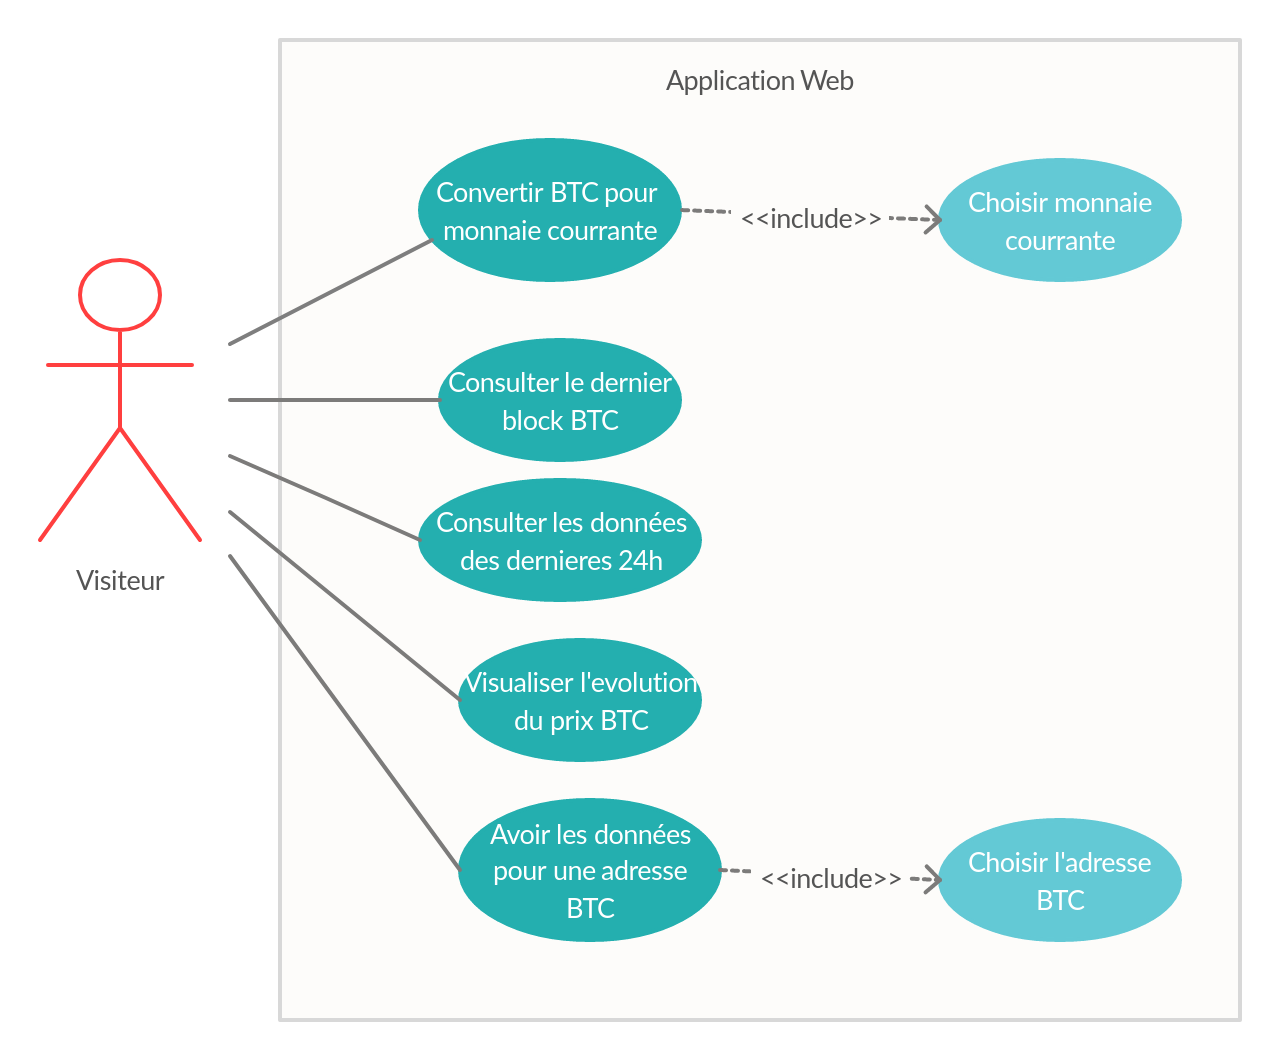
\includegraphics[width=6.94in,height=5.75in]{./media/image2.png}
\end{figure}



\par

\textit{fig1:\tab use-case diagram}\par


\vspace{\baselineskip}

\vspace{\baselineskip}

\vspace{\baselineskip}

\vspace{\baselineskip}

\vspace{\baselineskip}

\vspace{\baselineskip}
	\item 1.2\tab Diagramme de sequences :\par

Le projet propose l’utilisation d’un endpoint pour récuperer les données relatives au Bitcoin, en effet ce domaine, comme tout autre domaine de finance d’ailleurs, connait des changements permanents. Une façon pour récupérer des données actualisées est de connecter l’application à un endpoint auparavant à jour. Ainsi on a élaboré des diagrammes de séquence comme suivent:\par




\begin{figure}[H]
	\begin{Center}
		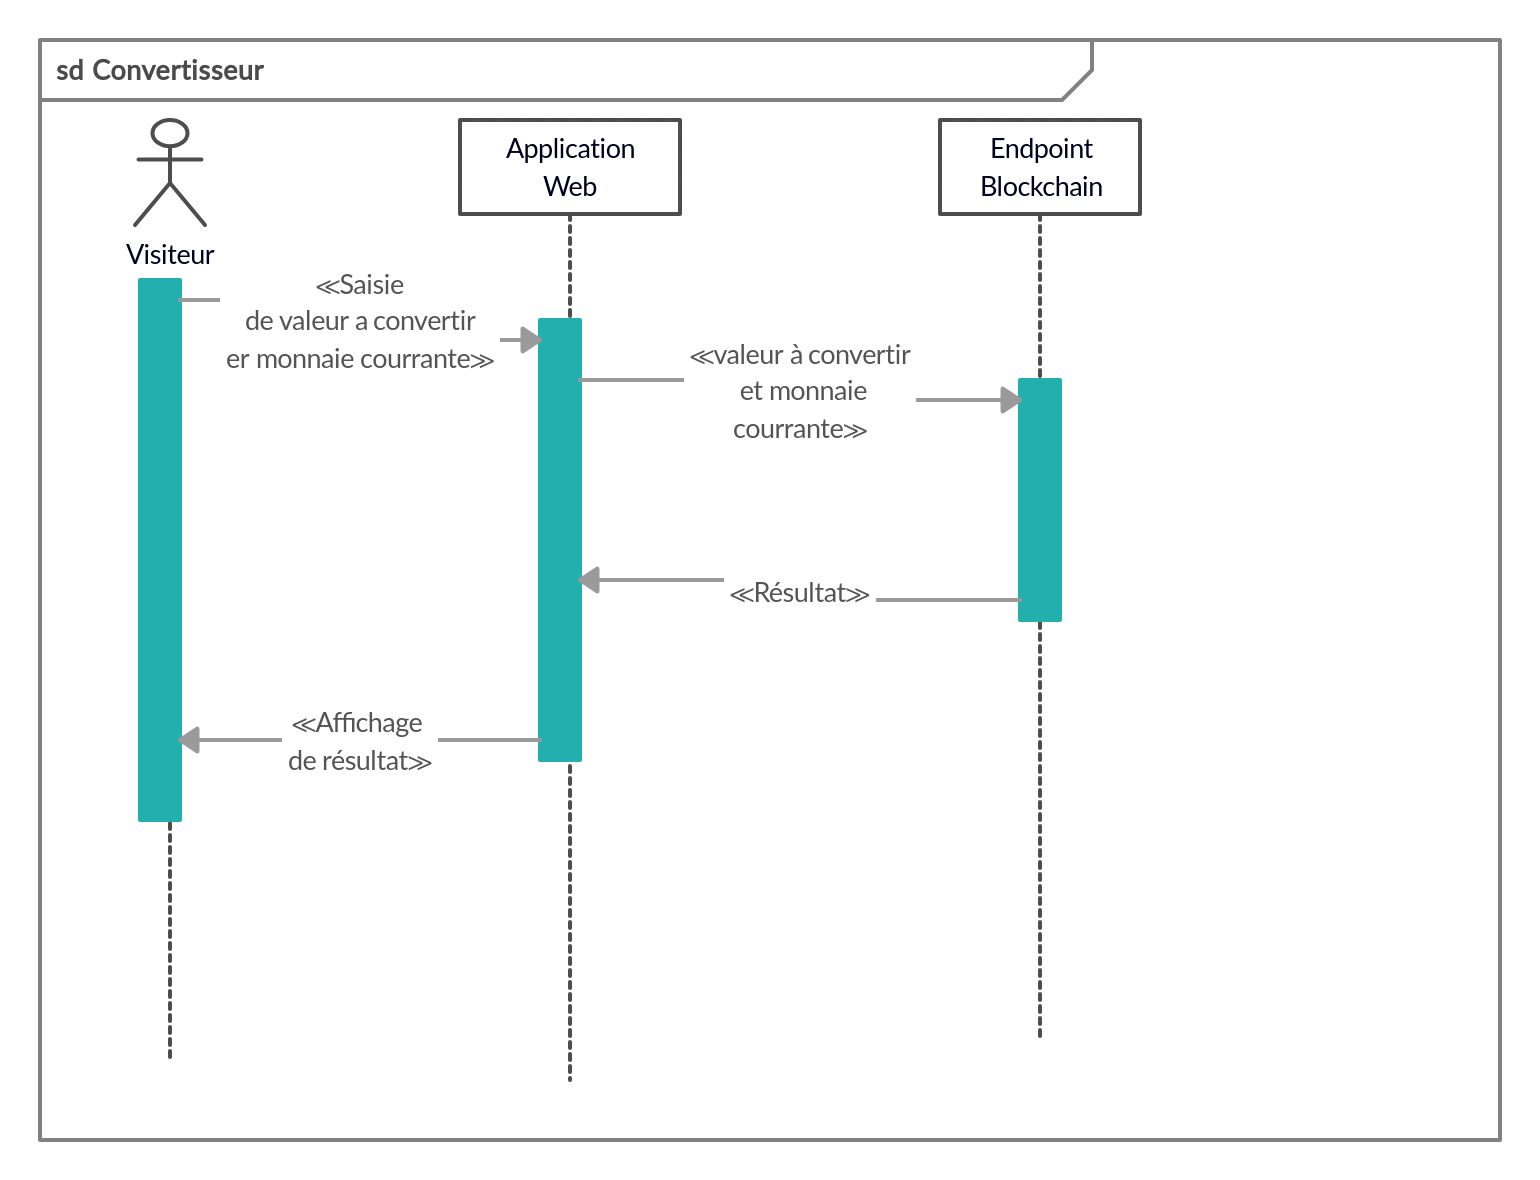
\includegraphics[width=6.69in,height=5.13in]{./media/image3.png}
	\end{Center}
\end{figure}



\textit{fig 2: sequence diagram pour convertisseur}\par


\vspace{\baselineskip}




\begin{figure}[H]
	\begin{Center}
		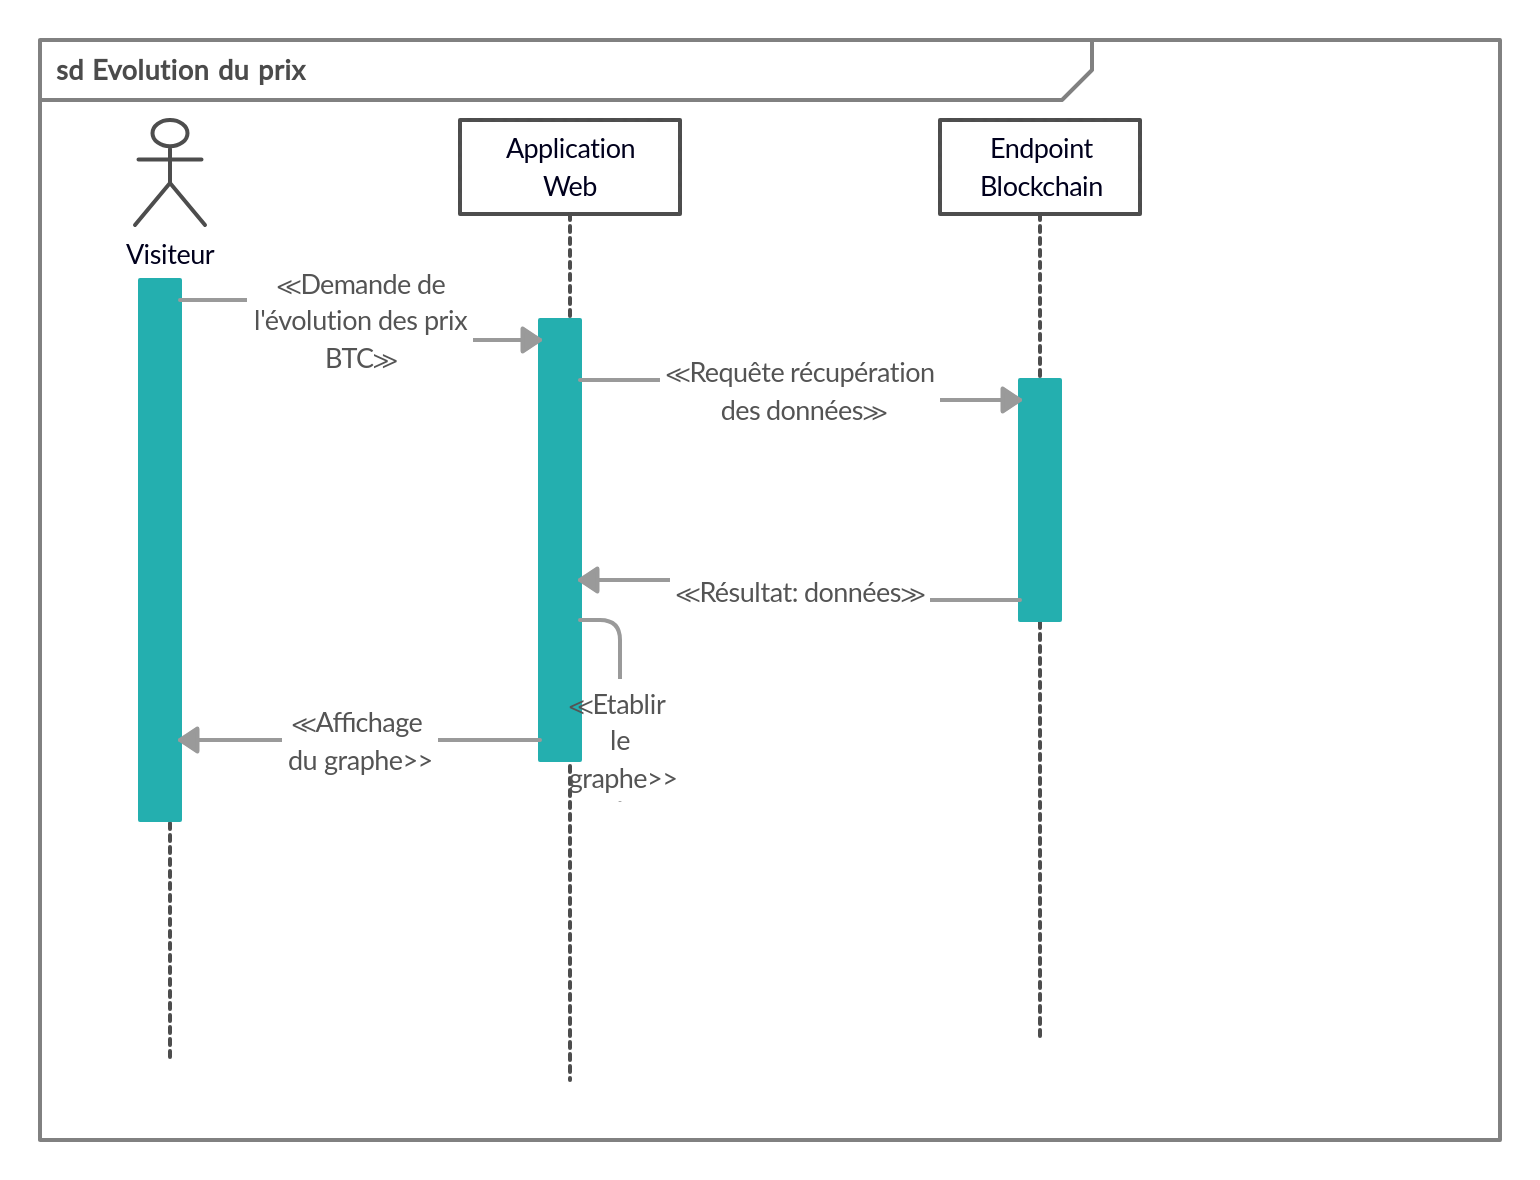
\includegraphics[width=6.69in,height=5.13in]{./media/image4.png}
	\end{Center}
\end{figure}




\textit{fig 3: sequence diagram pour la consultation de l’évolution des prix.}\par


\vspace{\baselineskip}

\vspace{\baselineskip}

\vspace{\baselineskip}
	\item 1. 3 Diagramme des classes (niveau conception):\par

Lors de la conception, la première idée fut d’utiliser le design pattern $``$Strategy$"$  au niveau du modèle (la notion modèle dans un contexte MVC), alors l’analyse a abouti à ce diagramme des classes:\par


\vspace{\baselineskip}

\vspace{\baselineskip}

\vspace{\baselineskip}

\vspace{\baselineskip}

\vspace{\baselineskip}

\vspace{\baselineskip}

\vspace{\baselineskip}




\begin{figure}[H]
\advance\leftskip 0.35in		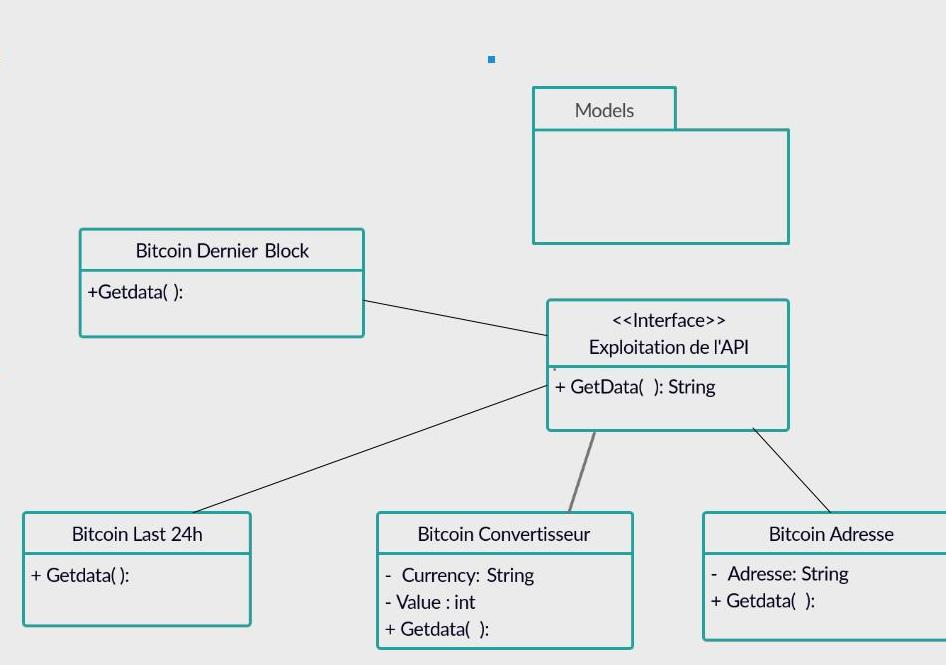
\includegraphics[width=5.52in,height=3.34in]{./media/image5.jpeg}
\end{figure}




\par


\vspace{\baselineskip}

\vspace{\baselineskip}

\vspace{\baselineskip}

\vspace{\baselineskip}

\vspace{\baselineskip}

\vspace{\baselineskip}

\vspace{\baselineskip}

\vspace{\baselineskip}

\vspace{\baselineskip}

\vspace{\baselineskip}
\textit{fig 4 : class-diagram pour le package Models: niveau conception}\par


\vspace{\baselineskip}

\vspace{\baselineskip}

\vspace{\baselineskip}
	\item Réalisation:\par

	\item 2.1 Etat de l’art:\par

\tab Le projet a été réalisé par l’environnement de développement: Intellij IDEA, qui est principalement destiné au développement Java. J’ai utilisé le conteneur Apache Tomcat, qui est connu pour son utilisation dans les projets manipulant les servlets et JSP.\par





\begin{figure}[H]
	\begin{Center}
		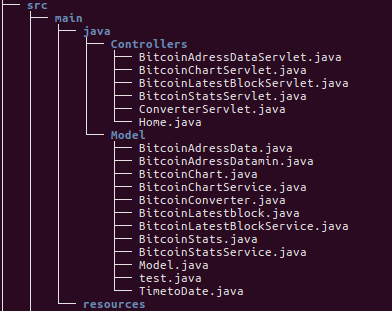
\includegraphics[width=3.81in,height=2.67in]{./media/image6.png}
	\end{Center}
\end{figure}




\par


\vspace{\baselineskip}

\vspace{\baselineskip}

\vspace{\baselineskip}

\vspace{\baselineskip}

\vspace{\baselineskip}

\vspace{\baselineskip}

\vspace{\baselineskip}

\vspace{\baselineskip}
\textit{fig 5: prise d’écran d’une partie de l’espace de travail.}\par

	\item 2.2\tab Diagramme des classes lors de la réalisation:\par

Le diagramme, établi lors de la conception, a subi quelques changements lors de la phase réalisation:\par


\vspace{\baselineskip}




\begin{figure}[H]
\advance\leftskip -0.07in		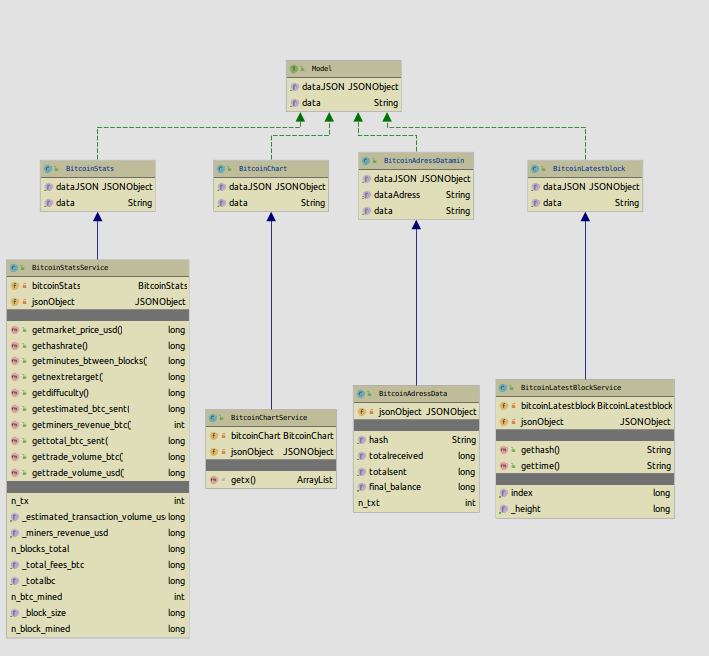
\includegraphics[width=6.69in,height=6.19in]{./media/image7.png}
\end{figure}




\textit{fig 6: class-diagram lors de la réalisation.}\par


\vspace{\baselineskip}
	\item 2.3\tab Prises d’écan de l’application web:\par

\begin{enumerate}
	\item Home Page:\par




\begin{figure}[H]
	\begin{Center}
		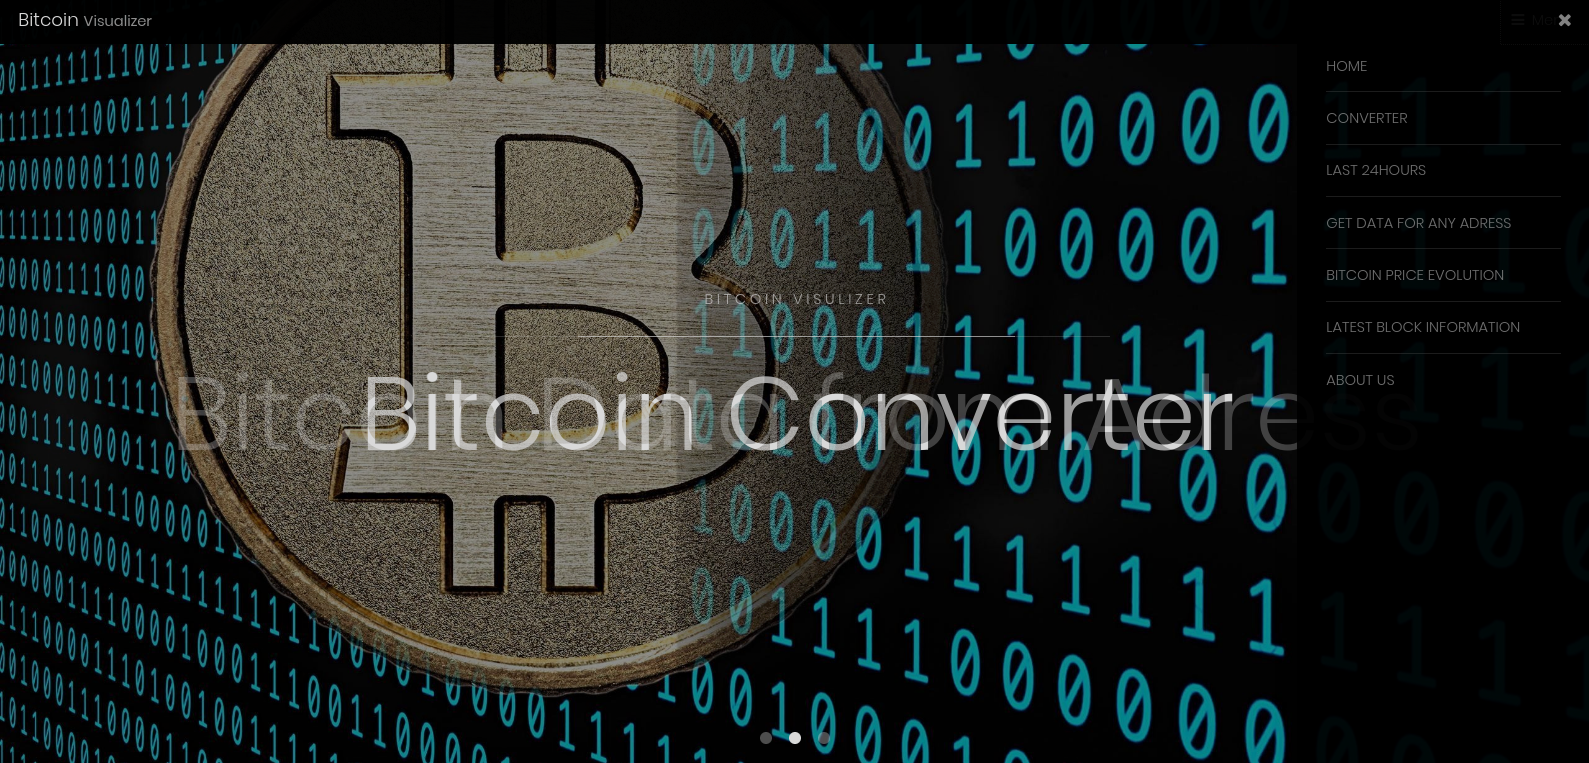
\includegraphics[width=6.69in,height=3.2in]{./media/image8.png}
	\end{Center}
\end{figure}




\par





\begin{figure}[H]
	\begin{Center}
		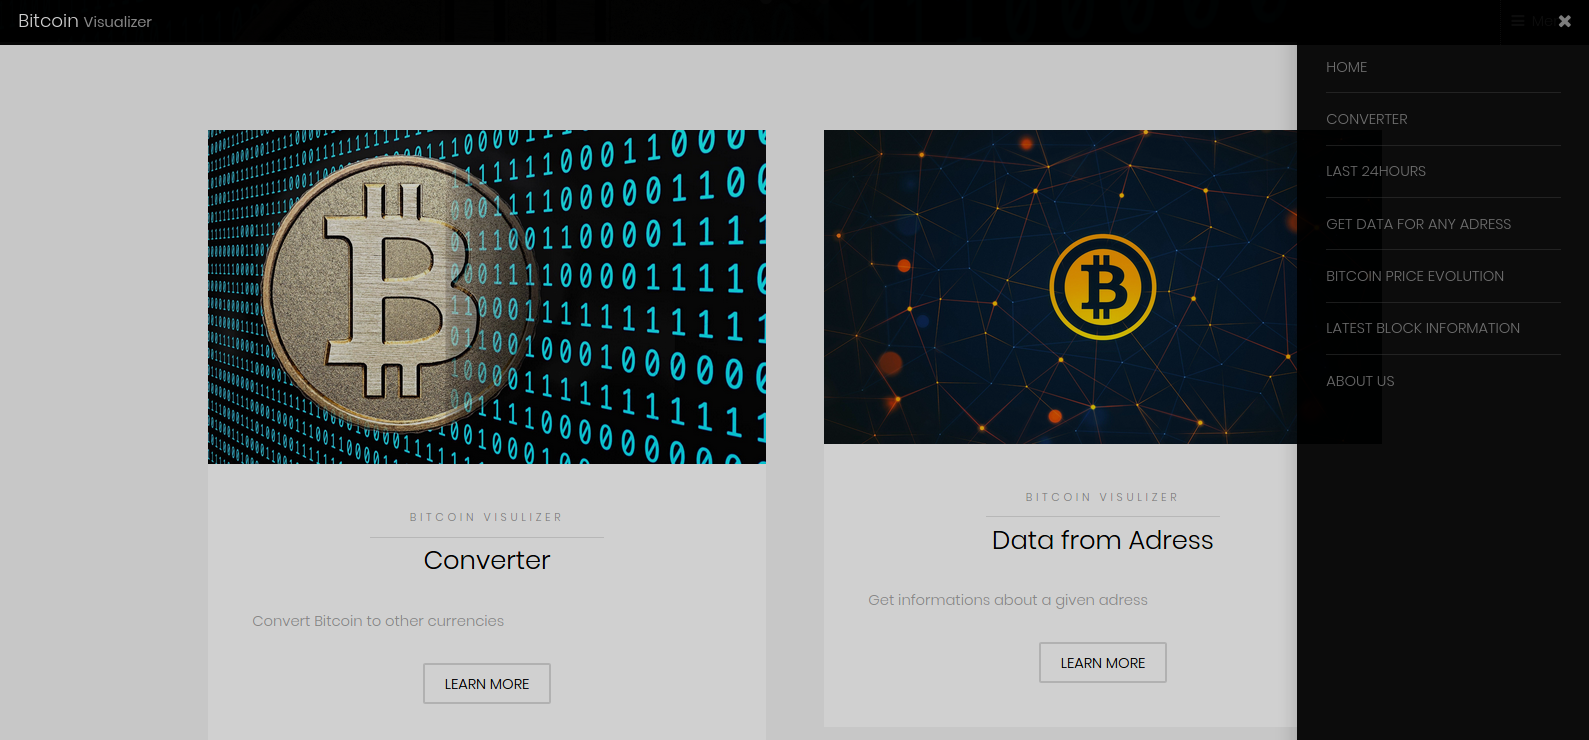
\includegraphics[width=6.69in,height=3.29in]{./media/image9.png}
	\end{Center}
\end{figure}



	\item \par

	\item Page Convertisseur:\par





\begin{figure}[H]
	\begin{Center}
		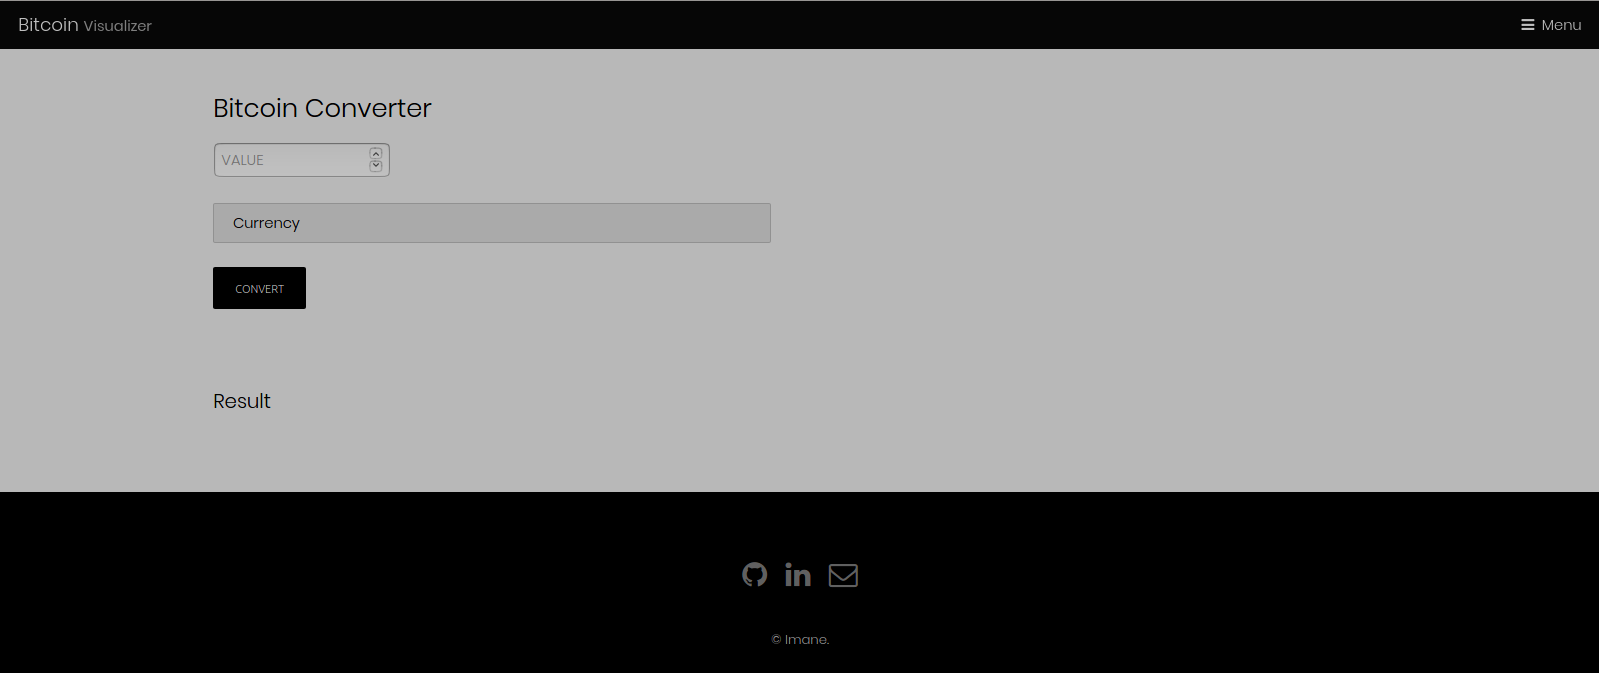
\includegraphics[width=6.69in,height=2.92in]{./media/image10.png}
	\end{Center}
\end{figure}




\par

	\item Page de l’évolution du prix Bitcoin:\par





\begin{figure}[H]
	\begin{Center}
		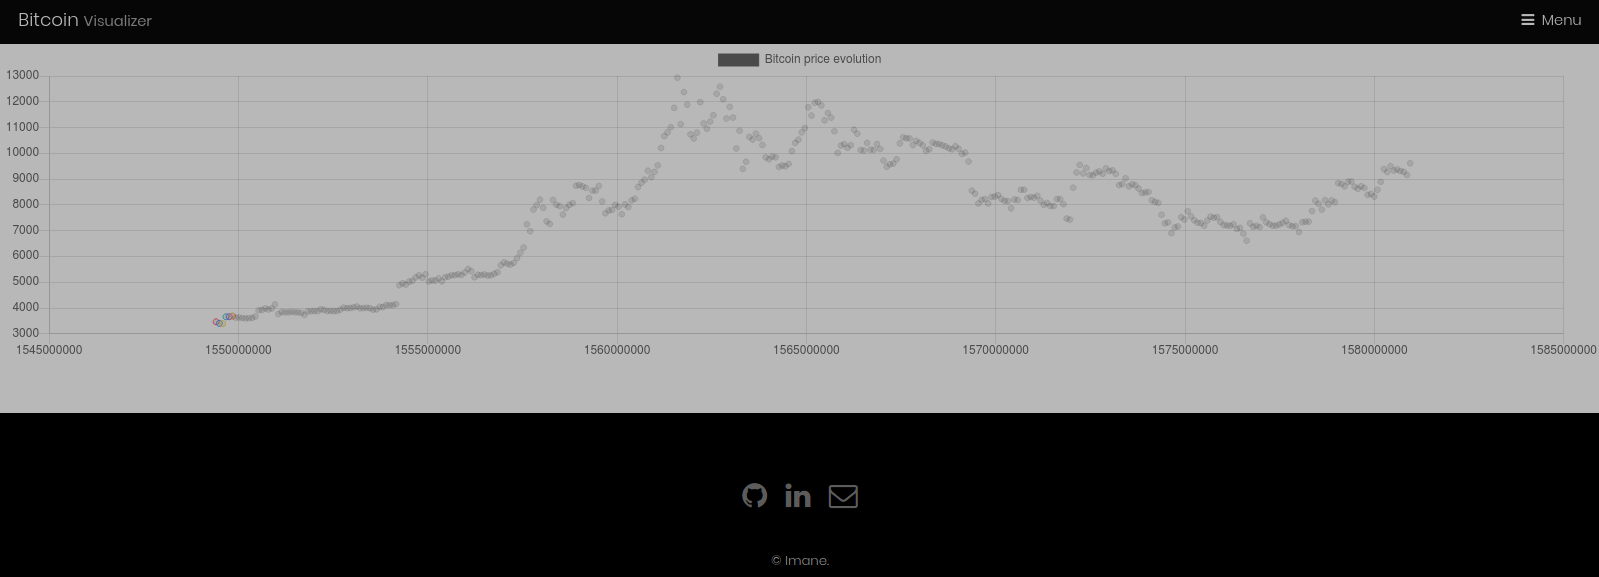
\includegraphics[width=6.69in,height=2.62in]{./media/image11.png}
	\end{Center}
\end{figure}




	\item \par

	\item Page de récupération des données pour une adresse:
\end{enumerate}
\end{enumerate}\par





\begin{figure}[H]
	\begin{Center}
		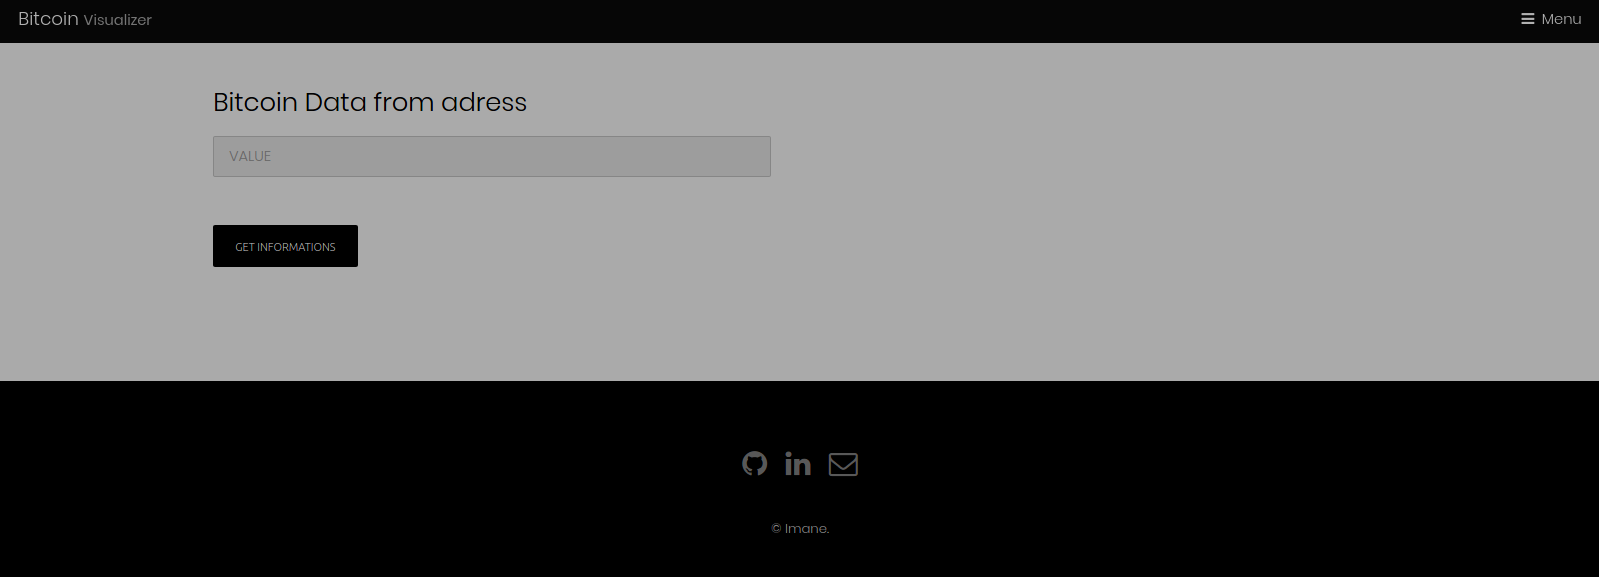
\includegraphics[width=6.69in,height=2.44in]{./media/image12.png}
	\end{Center}
\end{figure}




\par


\vspace{\baselineskip}

\vspace{\baselineskip}

\vspace{\baselineskip}

\vspace{\baselineskip}

\vspace{\baselineskip}

\vspace{\baselineskip}

\vspace{\baselineskip}

\vspace{\baselineskip}

\vspace{\baselineskip}

\vspace{\baselineskip}

\vspace{\baselineskip}
	\item Perspectives:\par

Je propose, à titre de perspective, d’ajouter le real time au site, notamment dans l’affaichage de l’évolution du prix; ainsi on élimine le besoin d’actualiser la page.\par

	\item Conclusion:\par


\vspace{\baselineskip}
En substance, ce projet consiste à développer une application Web pour la visualisation des données relatives au Bitcoin: convertisseur, évolution du prix, nouveautés$ \ldots $ \par

Ce projet m’a permis d’appliquer les connaissances inculquées au cours de mes études à l’ENSIAS: l’analyse, la conception, le modèle MVC, la technologie Java EE.\par


\vspace{\baselineskip}

\vspace{\baselineskip}

\vspace{\baselineskip}

\vspace{\baselineskip}

\vspace{\baselineskip}

\vspace{\baselineskip}

\vspace{\baselineskip}

\vspace{\baselineskip}

\vspace{\baselineskip}

\vspace{\baselineskip}

\vspace{\baselineskip}

\vspace{\baselineskip}

\vspace{\baselineskip}

\vspace{\baselineskip}

\vspace{\baselineskip}

\vspace{\baselineskip}

\vspace{\baselineskip}

\vspace{\baselineskip}

\vspace{\baselineskip}

\vspace{\baselineskip}

\vspace{\baselineskip}

\vspace{\baselineskip}
Bibliographie:\par

blockchain.info/\par

\href{http://shop.oreilly.com/product/9780596005726.do}{Java Servlet $\&$  JSP Cookbook - O'Reilly Media} par \href{http://www.oreillynet.com/pub/au/674}{Bruce Perry}\par

www.hcltech.com/technology-qa/what-is-api-integration\par


\vspace{\baselineskip}

\vspace{\baselineskip}
\setlength{\parskip}{6.96pt}

\end{enumerate}
\printbibliography
\end{document}
